%!TEX root = ms.tex

This appendix describes \py{cartesian.Diagram} and \py{PythonFunctor}, an
implementation of \emph{Lawvere theories} and their models.
We first give a short introduction to symmetric monoidal categories (SMC), PROPs and functorial semantics.

A (strict) monoidal category $\mathbf{C}$ is \emph{symmetric} when it comes equipped
with a natural transformation $\sigma_{x, y} : x \otimes y \to y \otimes x$
such that $\sigma_{y, x} \circ \sigma_{x, y} = 1_{x \otimes y}$ (involution)
and $\sigma_{x, y \otimes z} =
(1_{z} \otimes \sigma_{x, z}) \circ (\sigma_{x, y} \otimes 1_{z})$ (hexagon).
A component $\sigma_{x, y}$ is depicted as a swap of the wires for $x$ and $y$.
The free symmetric monoidal category $\mathbf{SMC}(\Sigma)$ generated by a monoidal
signature $\Sigma$ can be defined as a quotient $\mathbf{MC}(\Sigma') / \cal{S}$ of
the free monoidal category generated by the disjoint union
$\Sigma' = \Sigma + \set{\sigma_{x, y}}_{x, y \in \Sigma_0}$. The relation
$\cal{S}$ is generated by the rules for involution and naturality:
\begin{center}
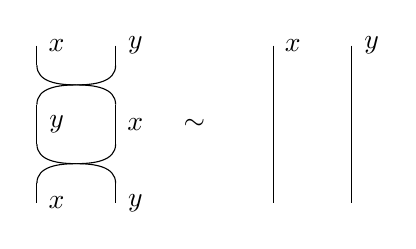
\begin{tikzpicture}[baseline=(O.base)]
\node (O) at (0, 1.0) {};
\node () at (0.25, 2.0) {$x$};
\node () at (1.25, 2.0) {$y$};
\node () at (0.25, 1.0) {$y$};
\node () at (1.25, 1.0) {$x$};
\node () at (0.25, 0.0) {$x$};
\node () at (1.25, 0.0) {$y$};
\draw [out=-90, in=90] (0, 2.0) to (0, 1.75);
\draw [out=-90, in=90] (1, 2.0) to (1, 1.75);
\draw [out=180, in=90] (0.5, 1.5) to (0.0, 1.25);
\draw [out=0, in=90] (0.5, 1.5) to (1.0, 1.25);
\draw [out=-90, in=180] (0, 1.75) to (0.5, 1.5);
\draw [out=-90, in=0] (1, 1.75) to (0.5, 1.5);
\draw [out=-90, in=90] (0.0, 1.25) to (0.0, 0.75);
\draw [out=-90, in=90] (1.0, 1.25) to (1.0, 0.75);
\draw [out=180, in=90] (0.5, 0.5) to (0.0, 0.25);
\draw [out=0, in=90] (0.5, 0.5) to (1.0, 0.25);
\draw [out=-90, in=180] (0.0, 0.75) to (0.5, 0.5);
\draw [out=-90, in=0] (1.0, 0.75) to (0.5, 0.5);
\draw [out=-90, in=90] (0.0, 0.25) to (0.0, 0.0);
\draw [out=-90, in=90] (1.0, 0.25) to (1.0, 0.0);
\node () at (2, 1.0) {$\sim$};
\node () at (3.25, 2.0) {$x$};
\node () at (4.25, 2.0) {$y$};
\draw [out=-90, in=90] (3, 2.0) to (3, 0.0);
\draw [out=-90, in=90] (4, 2.0) to (4, 0.0);
\end{tikzpicture}

\qquad and \qquad \quad
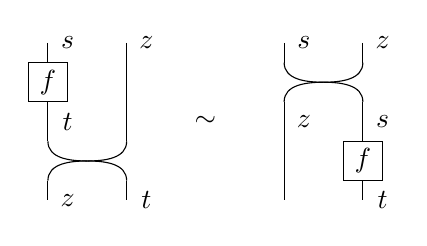
\begin{tikzpicture}[baseline=(O.base)]
\node (O) at (0, 1.0) {};
\node () at (0.25, 2.0) {$s$};
\node () at (1.25, 2.0) {$z$};
\node () at (0.25, 1.0) {$t$};
\node () at (0.25, 0.0) {$z$};
\node () at (1.25, 0.0) {$t$};
\draw [out=-90, in=90] (0, 2.0) to (0, 1.75);
\draw [out=-90, in=90] (1, 2.0) to (1, 0.75);
\draw [out=-90, in=90] (0.0, 1.25) to (0.0, 0.75);
\draw [out=180, in=90] (0.5, 0.5) to (0.0, 0.25);
\draw [out=0, in=90] (0.5, 0.5) to (1.0, 0.25);
\draw [out=-90, in=180] (0.0, 0.75) to (0.5, 0.5);
\draw [out=-90, in=0] (1, 0.75) to (0.5, 0.5);
\draw [out=-90, in=90] (0.0, 0.25) to (0.0, 0.0);
\draw [out=-90, in=90] (1.0, 0.25) to (1.0, 0.0);
\draw (-0.25, 1.25) -- (0.25, 1.25) -- (0.25, 1.75) -- (-0.25, 1.75) -- (-0.25, 1.25);
\node () at (0.0, 1.5) {$f$};
\node () at (2, 1.0) {$\sim$};
\node () at (3.25, 2.0) {$s$};
\node () at (4.25, 2.0) {$z$};
\node () at (3.25, 1.0) {$z$};
\node () at (4.25, 1.0) {$s$};
\node () at (4.25, 0.0) {$t$};
\draw [out=-90, in=90] (3, 2.0) to (3, 1.75);
\draw [out=-90, in=90] (4, 2.0) to (4, 1.75);
\draw [out=180, in=90] (3.5, 1.5) to (3.0, 1.25);
\draw [out=0, in=90] (3.5, 1.5) to (4.0, 1.25);
\draw [out=-90, in=180] (3, 1.75) to (3.5, 1.5);
\draw [out=-90, in=0] (4, 1.75) to (3.5, 1.5);
\draw [out=-90, in=90] (3.0, 1.25) to (3.0, 0.0);
\draw [out=-90, in=90] (4.0, 1.25) to (4.0, 0.75);
\draw [out=-90, in=90] (4.0, 0.25) to (4.0, 0.0);
\draw (3.75, 0.25) -- (4.25, 0.25) -- (4.25, 0.75) -- (3.75, 0.75) -- (3.75, 0.25);
\node () at (4.0, 0.5) {$f$};
\end{tikzpicture}

\end{center}
for all $x, y, z \in \Sigma_0$ and $f : s \to t$ in $\Sigma'$. Note that
$s, t \in \Sigma_0^\star$ may be of arbitrary length, in which case $\sigma_{s, z}$ and $\sigma_{t, z}$ are defined as ladders of swaps,
i.e. the symmetry for compound types $\sigma_{x \otimes y, z}$ and
$\sigma_{x, y \otimes z}$ is defined inductively by:
\begin{center}
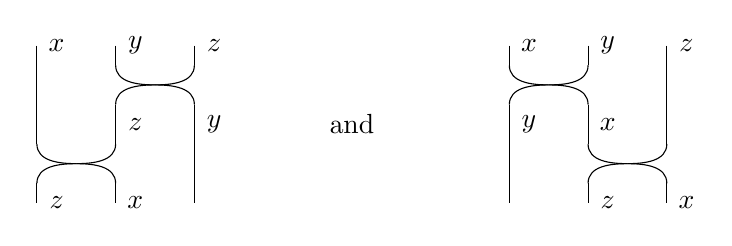
\begin{tikzpicture}[baseline=(O.base)]
\node (O) at (0, 1.0) {};
\node () at (0.25, 2.0) {$x$};
\node () at (1.25, 2.0) {$y$};
\node () at (2.25, 2.0) {$z$};
\node () at (1.25, 1.0) {$z$};
\node () at (2.25, 1.0) {$y$};
\node () at (0.25, 0.0) {$z$};
\node () at (1.25, 0.0) {$x$};
\draw [out=-90, in=90] (0, 2.0) to (0, 0.75);
\draw [out=-90, in=90] (1, 2.0) to (1, 1.75);
\draw [out=-90, in=90] (2, 2.0) to (2, 1.75);
\draw [out=180, in=90] (1.5, 1.5) to (1.0, 1.25);
\draw [out=0, in=90] (1.5, 1.5) to (2.0, 1.25);
\draw [out=-90, in=180] (1, 1.75) to (1.5, 1.5);
\draw [out=-90, in=0] (2, 1.75) to (1.5, 1.5);
\draw [out=-90, in=90] (1.0, 1.25) to (1.0, 0.75);
\draw [out=-90, in=90] (2.0, 1.25) to (2.0, 0.0);
\draw [out=180, in=90] (0.5, 0.5) to (0.0, 0.25);
\draw [out=0, in=90] (0.5, 0.5) to (1.0, 0.25);
\draw [out=-90, in=180] (0, 0.75) to (0.5, 0.5);
\draw [out=-90, in=0] (1.0, 0.75) to (0.5, 0.5);
\draw [out=-90, in=90] (0.0, 0.25) to (0.0, 0.0);
\draw [out=-90, in=90] (1.0, 0.25) to (1.0, 0.0);
\node () at (4, 1.0) {and};
\node () at (6.25, 2.0) {$x$};
\node () at (7.25, 2.0) {$y$};
\node () at (8.25, 2.0) {$z$};
\node () at (6.25, 1.0) {$y$};
\node () at (7.25, 1.0) {$x$};
\node () at (7.25, 0.0) {$z$};
\node () at (8.25, 0.0) {$x$};
\draw [out=-90, in=90] (6, 2.0) to (6, 1.75);
\draw [out=-90, in=90] (7, 2.0) to (7, 1.75);
\draw [out=-90, in=90] (8, 2.0) to (8, 0.75);
\draw [out=180, in=90] (6.5, 1.5) to (6.0, 1.25);
\draw [out=0, in=90] (6.5, 1.5) to (7.0, 1.25);
\draw [out=-90, in=180] (6, 1.75) to (6.5, 1.5);
\draw [out=-90, in=0] (7, 1.75) to (6.5, 1.5);
\draw [out=-90, in=90] (6.0, 1.25) to (6.0, 0.0);
\draw [out=-90, in=90] (7.0, 1.25) to (7.0, 0.75);
\draw [out=180, in=90] (7.5, 0.5) to (7.0, 0.25);
\draw [out=0, in=90] (7.5, 0.5) to (8.0, 0.25);
\draw [out=-90, in=180] (7.0, 0.75) to (7.5, 0.5);
\draw [out=-90, in=0] (8, 0.75) to (7.5, 0.5);
\draw [out=-90, in=90] (7.0, 0.25) to (7.0, 0.0);
\draw [out=-90, in=90] (8.0, 0.25) to (8.0, 0.0);
\end{tikzpicture}

\end{center}
The symmetry for the empty type is defined to be the identity
$\sigma_{x, 1} = \sigma_{1, x} = 1_x$.
% Thus, the hexagon identity holds on the nose. Picking $f = \sigma_{x, y}$ in
% the naturality rule yields the Yang-Baxter identity:
% \begin{center}
% 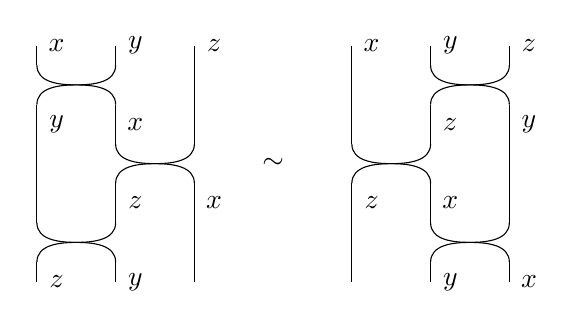
\begin{tikzpicture}[baseline=(O.base)]
\node (O) at (0, 1.5) {};
\node () at (0.25, 3.0) {$x$};
\node () at (1.25, 3.0) {$y$};
\node () at (2.25, 3.0) {$z$};
\node () at (0.25, 2.0) {$y$};
\node () at (1.25, 2.0) {$x$};
\node () at (1.25, 1.0) {$z$};
\node () at (2.25, 1.0) {$x$};
\node () at (0.25, 0.0) {$z$};
\node () at (1.25, 0.0) {$y$};
\draw [out=-90, in=90] (0, 3.0) to (0, 2.75);
\draw [out=-90, in=90] (1, 3.0) to (1, 2.75);
\draw [out=-90, in=90] (2, 3.0) to (2, 1.75);
\draw [out=180, in=90] (0.5, 2.5) to (0.0, 2.25);
\draw [out=0, in=90] (0.5, 2.5) to (1.0, 2.25);
\draw [out=-90, in=180] (0, 2.75) to (0.5, 2.5);
\draw [out=-90, in=0] (1, 2.75) to (0.5, 2.5);
\draw [out=-90, in=90] (0.0, 2.25) to (0.0, 0.75);
\draw [out=-90, in=90] (1.0, 2.25) to (1.0, 1.75);
\draw [out=180, in=90] (1.5, 1.5) to (1.0, 1.25);
\draw [out=0, in=90] (1.5, 1.5) to (2.0, 1.25);
\draw [out=-90, in=180] (1.0, 1.75) to (1.5, 1.5);
\draw [out=-90, in=0] (2, 1.75) to (1.5, 1.5);
\draw [out=-90, in=90] (1.0, 1.25) to (1.0, 0.75);
\draw [out=-90, in=90] (2.0, 1.25) to (2.0, 0.0);
\draw [out=180, in=90] (0.5, 0.5) to (0.0, 0.25);
\draw [out=0, in=90] (0.5, 0.5) to (1.0, 0.25);
\draw [out=-90, in=180] (0.0, 0.75) to (0.5, 0.5);
\draw [out=-90, in=0] (1.0, 0.75) to (0.5, 0.5);
\draw [out=-90, in=90] (0.0, 0.25) to (0.0, 0.0);
\draw [out=-90, in=90] (1.0, 0.25) to (1.0, 0.0);
\node () at (3, 1.5) {$\sim$};
\node () at (4.25, 3.0) {$x$};
\node () at (5.25, 3.0) {$y$};
\node () at (6.25, 3.0) {$z$};
\node () at (5.25, 2.0) {$z$};
\node () at (6.25, 2.0) {$y$};
\node () at (4.25, 1.0) {$z$};
\node () at (5.25, 1.0) {$x$};
\node () at (5.25, 0.0) {$y$};
\node () at (6.25, 0.0) {$x$};
\draw [out=-90, in=90] (4, 3.0) to (4, 1.75);
\draw [out=-90, in=90] (5, 3.0) to (5, 2.75);
\draw [out=-90, in=90] (6, 3.0) to (6, 2.75);
\draw [out=180, in=90] (5.5, 2.5) to (5.0, 2.25);
\draw [out=0, in=90] (5.5, 2.5) to (6.0, 2.25);
\draw [out=-90, in=180] (5, 2.75) to (5.5, 2.5);
\draw [out=-90, in=0] (6, 2.75) to (5.5, 2.5);
\draw [out=-90, in=90] (5.0, 2.25) to (5.0, 1.75);
\draw [out=-90, in=90] (6.0, 2.25) to (6.0, 0.75);
\draw [out=180, in=90] (4.5, 1.5) to (4.0, 1.25);
\draw [out=0, in=90] (4.5, 1.5) to (5.0, 1.25);
\draw [out=-90, in=180] (4, 1.75) to (4.5, 1.5);
\draw [out=-90, in=0] (5.0, 1.75) to (4.5, 1.5);
\draw [out=-90, in=90] (4.0, 1.25) to (4.0, 0.0);
\draw [out=-90, in=90] (5.0, 1.25) to (5.0, 0.75);
\draw [out=180, in=90] (5.5, 0.5) to (5.0, 0.25);
\draw [out=0, in=90] (5.5, 0.5) to (6.0, 0.25);
\draw [out=-90, in=180] (5.0, 0.75) to (5.5, 0.5);
\draw [out=-90, in=0] (6.0, 0.75) to (5.5, 0.5);
\draw [out=-90, in=90] (5.0, 0.25) to (5.0, 0.0);
\draw [out=-90, in=90] (6.0, 0.25) to (6.0, 0.0);
\end{tikzpicture}

% \end{center}
An SMC where the tensor is the Cartesian product and the unit is terminal
(i.e. a category with finite products) is called a \emph{Cartesian category}.
Equivalently, an SMC is Cartesian when objects carry a natural
commutative comonoid structure \cite[6.1]{Selinger10}.
Given a monoidal signature $\Sigma$, the free Cartesian category
$\mathbf{CC}(\Sigma)$ is the quotient
$\mathbf{MC}(\Sigma'') / (\cal{S} + \cal{P})$ for
$\Sigma'' = \Sigma' + \set{\mu_{x} : x \to x \otimes x}_{x \in \Sigma_0} + \set{\epsilon_x : x \to 1}_{x \in \Sigma_0}$.
The components $\mu_{x}$ and $\epsilon_{x}$ are depicted as wire splitting and
ending respectively. The comonoids of non-atomic
types inductively. That for the unit is the identity and the comonoid
of $x \otimes y$ is given by:
\begin{center}
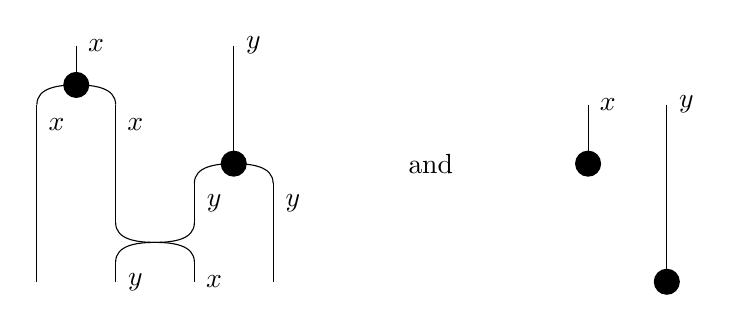
\begin{tikzpicture}[baseline=(O.base)]
\node (O) at (0, 1.5) {};
\node () at (0.75, 3.0) {$x$};
\node () at (2.75, 3.0) {$y$};
\node () at (0.25, 2.0) {$x$};
\node () at (1.25, 2.0) {$x$};
\node () at (2.25, 1.0) {$y$};
\node () at (3.25, 1.0) {$y$};
\node () at (1.25, 0.0) {$y$};
\node () at (2.25, 0.0) {$x$};
\draw [out=-90, in=90] (0.5, 3.0) to (0.5, 2.75);
\draw [out=-90, in=90] (2.5, 3.0) to (2.5, 1.75);
\draw [out=180, in=90] (0.5, 2.5) to (0.0, 2.25);
\draw [out=0, in=90] (0.5, 2.5) to (1.0, 2.25);
\draw [out=-90, in=90] (0.5, 2.75) to (0.5, 2.5);
\draw [out=-90, in=90] (0.0, 2.25) to (0.0, 0.0);
\draw [out=-90, in=90] (1.0, 2.25) to (1.0, 0.75);
\draw [out=180, in=90] (2.5, 1.5) to (2.0, 1.25);
\draw [out=0, in=90] (2.5, 1.5) to (3.0, 1.25);
\draw [out=-90, in=90] (2.5, 1.75) to (2.5, 1.5);
\draw [out=-90, in=90] (2.0, 1.25) to (2.0, 0.75);
\draw [out=-90, in=90] (3.0, 1.25) to (3.0, 0.0);
\draw [out=180, in=90] (1.5, 0.5) to (1.0, 0.25);
\draw [out=0, in=90] (1.5, 0.5) to (2.0, 0.25);
\draw [out=-90, in=180] (1.0, 0.75) to (1.5, 0.5);
\draw [out=-90, in=0] (2.0, 0.75) to (1.5, 0.5);
\draw [out=-90, in=90] (1.0, 0.25) to (1.0, 0.0);
\draw [out=-90, in=90] (2.0, 0.25) to (2.0, 0.0);
\node [circle, fill=black] () at (0.5, 2.5) {};
\node [circle, fill=black] () at (2.5, 1.5) {};
\node () at (5.0, 1.5) {and};
\node () at (7.25, 2.25) {$x$};
\node () at (8.25, 2.25) {$y$};
\draw [out=-90, in=90] (7.0, 2.25) to (7.0, 1.75);
\draw [out=-90, in=90] (8.0, 2.25) to (8.0, 0.25);
\draw [out=-90, in=90] (7.0, 1.75) to (7.0, 1.5);
\draw [out=-90, in=90] (8.0, 0.25) to (8.0, 0.0);
\node [circle, fill=black] () at (7.0, 1.5) {};
\node [circle, fill=black] () at (8.0, 0.0) {};
\end{tikzpicture}

\end{center}
The relation $(\cal{S} + \cal{P})$ is given by the axioms for commutative
comonoids plus naturality of symmetry, coproduct and counit for each generating
arrow.
A \emph{PROP} (PROduct and Permutation) \cite{Lack04} is an SMC generated by one object, a \emph{Lawvere theory} \cite{Lawvere63} is a Cartesian category generated one object.

Lawvere theories are implemented by the class \py{cartesian.Diagram}, a subclass of \linebreak \py{monoidal.Diagram} with static methods \py{swap}, \py{copy} and \py{delete} implementing the structural morphisms.
\py{cartesian.Box} is a subclass of \py{monoidal.Box} where each instance holds a Python function with natural numbers as domain and codomain. A Cartesian box \py{f} with \py{f.dom, f.cod == (m, n)} sends $m$-tuples to $n$-tuples, it can be defined in the standard syntax for Python functions using the decorator \py{@disco(m, n)}.
\py{Swap}, \py{Copy} and \py{Del} are subclasses of \py{cartesian.Box} which implement the symmetry and comonoid on the generating object.
\py{cartesian.Functor} is a subclass of \py{monoidal.Functor} which preserves symmetry and product.
\py{Function} is a subclass of \py{cartesian.Box} where \py{then} and \py{tensor} are overriden by function composition and tuple concatenation.
The \py{PythonFunctor} class implements Cartesian functors into \py{Function}, i.e. it maps the formal composition of diagrams to the concrete composition of functions.
Note that when \py{f} and \py{g} have side-effects, the tensor \py{f @ g} is in
general different from \py{Id(f.dom) @ g >> f @ Id(g.cod)}. Thus, \py{Function}
is closer to the implementation of a premonoidal than a monoidal category,
see example~\ref{example-2}.

\begin{example}
The Lawvere theory $\mathbf{F}$ with no generating arrows is the
opposite of the category of finite sets with disjoint union as monoidal structure: diagrams $f : m \to n$ in
$\mathbf{F}$ correspond precisely to the graphs of the functions $f : [n] \to [m]$.
The subcategories of diagrams in $\mathbf{F}$ with no coproduct, no counit and no symmetry correspond to injective, surjective and monotone functions respectively.
The subcategory of $\mathbf{F}$ generated by symmetry alone, i.e. the free SMC generated by one object, corresponds to bijections.
The normal form for diagrams in $\mathbf{F}$ is given by decomposing any function into a surjection and a monotone injection, see \cite[Theorem~3]{Lafont03}.
\end{example}

\begin{example}
For a semiring $\bb{S}$, the category of matrices over $\bb{S}$ with direct sum as monoidal product can be defined as a Lawvere theory generated by a commutative monoid $+ : 2 \to 1$ with unit $e : 0 \to 1$ and scalars $\set{s : 1 \to 1}_{s \in \bb{S}}$.
The relations are given by the axioms for semirings, see \cite{WadsleyWoods15}.
The naturality relation for the comonoid with respect to $+$ and $e$ are called the bialgebra laws, they have applications in control and network theory \cite{BaezErbele14,BaezEtAl18}.
\end{example}

\begin{example}
Let $\mathbf{NN}$ be the Lawvere
theory generated by sum $+ : 2 \to 1$, activation $a : 1 \to 1$,
finite sets of weights $\set{w_i : 1 \to 1}_{i \in W}$ and biases
$\set{b_i : 0 \to 1}_{i \in B}$. The arrows of $\mathbf{NN}$ are the diagrams
of neural network architectures.
Given a set of parameters $\theta : W + B \to \bb{R}$, an implementation is
given by the model $F_\theta : \mathbf{NN} \to \mathbf{Set}$ such that
$F_\theta(1) = \bb{R}$,
$F_\theta(b_i) = \set{() \mapsto \theta(b_i)}$,
$F_\theta(w_i) = \set{x \mapsto \theta(w_i) \cdot x}$,
$F_\theta(+) = \set{(x, y) \mapsto x + y}$
and $F_\theta(a) : \bb{R} \to \bb{R}$ is a non-linearity such as sigmoid.
A loss $l : (\bb{R}^m \to \bb{R}^n) \to \bb{R}$ for an architecture $f : m \to n$ in $\mathbf{NN}$ takes an implementation and
returns a real number encoding its success at some data-driven task.
The gradient of $\theta \mapsto l(F_\theta(f))$ can be computed by
back-propagation over the architecture $f$, using automatic differentiation tools such as $\mathtt{jax}$ \cite{Google/jax20}. The back-propagation algorithm is
itself part of a functor $\mathbf{NN} \to \mathbf{Learn}$, where $\mathbf{Learn}$ is a
Cartesian category of supervised learning algorithms, see \cite{FongEtAl17, FongJohnson19}.
\end{example}
